\documentclass{article}
\usepackage{graphicx}
\usepackage{titletoc}
\usepackage{titlesec}
\usepackage{geometry} 
\usepackage{fontspec, xunicode, xltxtra}
\usepackage{float}
\usepackage{cite}
\usepackage{amsmath}
\usepackage{listings}
\usepackage{titletoc}

\geometry{left=3cm,right=3cm,top=3cm,bottom=3cm}
\DeclareMathOperator*{\argmin}{argmin}
\DeclareMathOperator*{\argmax}{argmax}
\DeclareMathOperator*{\var}{var}
\DeclareMathOperator*{\expec}{E}

\begin{document}
\title{\textsf{Homework 1 for Pattern Recognition}}
\author{Fan JIN\quad (2015011506)}
\maketitle

\section*{Question 1}
{
    It is equivalent to prove $R^2 = r^2$ and to prove $$\sum_1^n (\bar{y} - \hat{y}_i)^2 \cdot \sum_1^n (\bar{x} - x_i)^2 = (\sum_1^n (\bar{x} - x_i)(\bar{y} - y_i))^2,$$

    With $\hat{y}_i = b x_i + \bar{y} - b \bar{x}$, we have the left-hand side
    $$\sum_1^n (\bar{y} - \hat{y}_i)^2 \cdot \sum_1^n (\bar{x} - x_i)^2 = b^2 \cdot (\sum_1^n (\bar{x} - x_i)^2)^2.$$

    Since the regression coefficient $$b = \frac{\sum_1^n (\bar{x} - x_i)(\bar{y} - y_i)}{\sum_1^n (\bar{x} - x_i)^2},$$ plug it in and we find the left-hand side equals the right-hand side. Thus, the equation above is proved.
}

\section*{Question 2}
{
    \subsection*{Case 1: $N=10$, $\sigma = 0.5$}
    {
        Linear model: $$\hat{y} = 5.9758 + 3.0841x ,\quad R^2 = 0.9963$$
        Quadratic model: $$\hat{y} = 5.9826 + 3.0843x - 0.0047x^2 ,\quad R^2 = 0.9963$$
        Cubic model: $$\hat{y} = 5.9864 + 2.9573x + 0.0045x^2 + 0.0356x^3 ,\quad R^2 = 0.9965$$

        \begin{figure}[H]
            \centering
            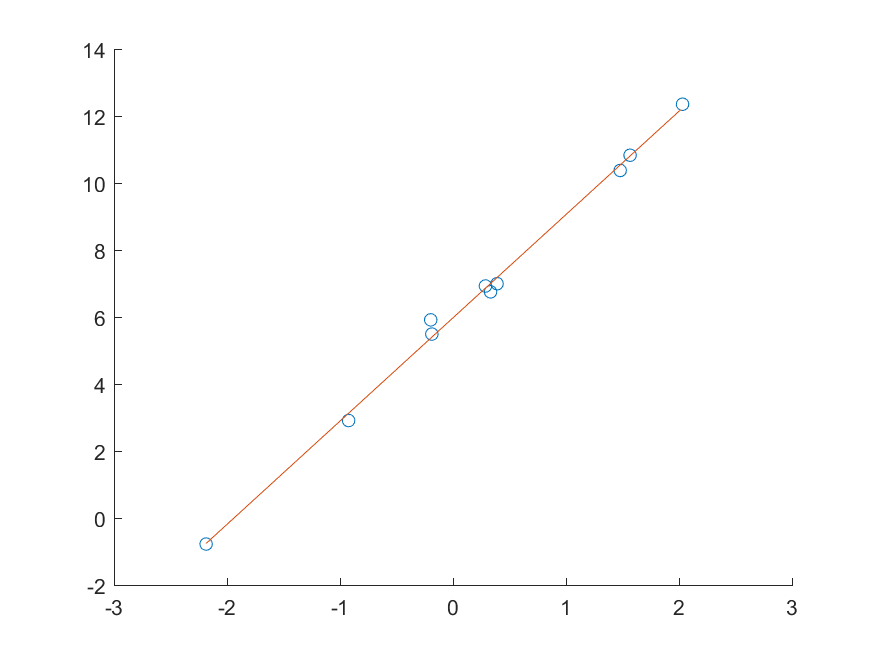
\includegraphics[width = 0.6\linewidth]{2-2-linear-10-0.5.png}
            \caption{Linear}
        \end{figure}

        \begin{figure}[H]
            \centering
            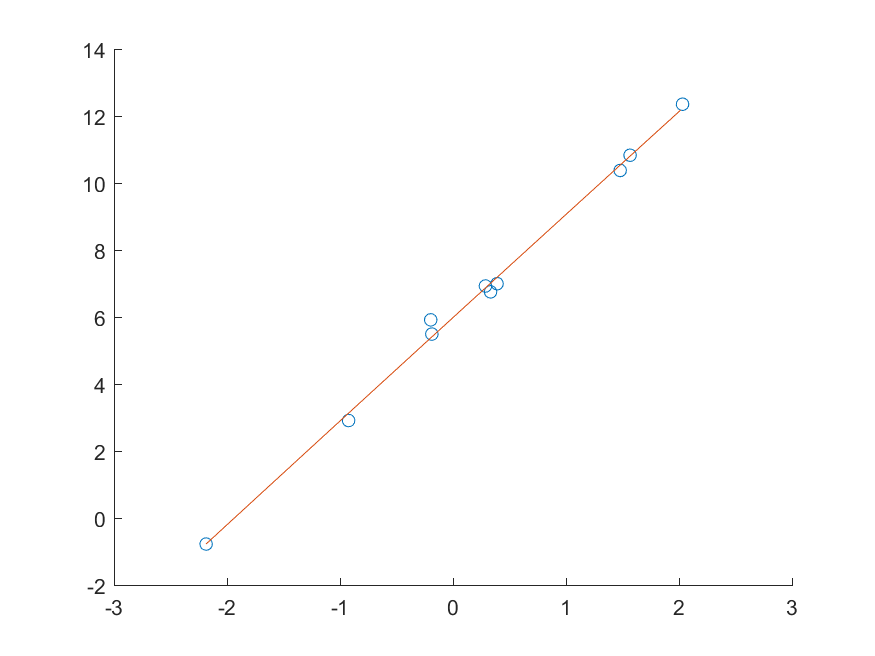
\includegraphics[width = 0.6\linewidth]{2-2-quadratic-10-0.5.png}
            \caption{Quadratic}
        \end{figure}

        \begin{figure}[H]
            \centering
            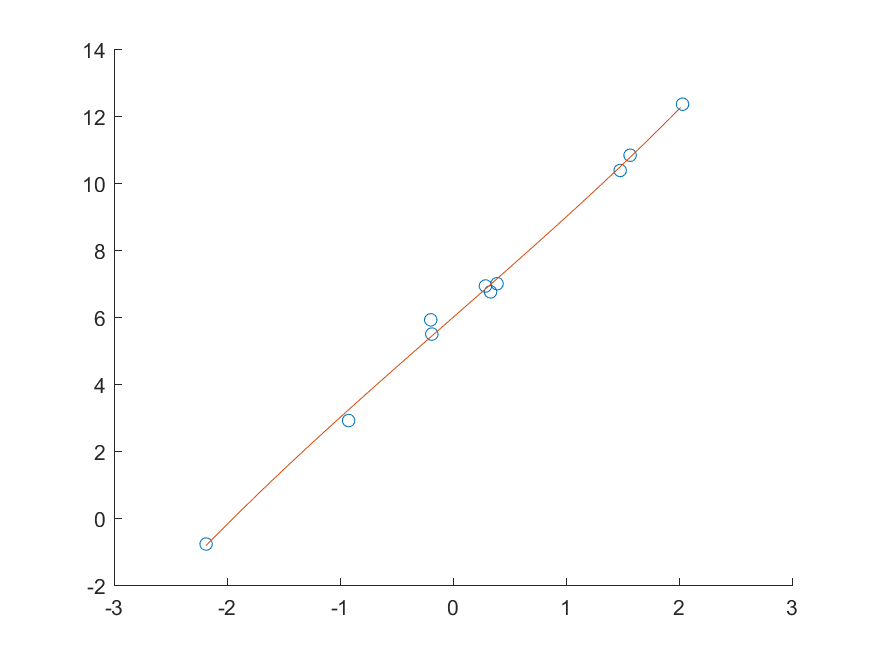
\includegraphics[width = 0.6\linewidth]{2-2-cubic-10-0.5.png}
            \caption{Cubic}
        \end{figure}

        Linear model (on testing set): $$\mathrm{RSS} = 7.4800, \quad \mathrm{RSS}/\mathrm{TSS} = 0.0018$$

        Quadratic model (on testing set): $$\mathrm{RSS} = 7.4650, \quad \mathrm{RSS}/\mathrm{TSS} = 0.0017$$

        Cubic model (on testing set): $$\mathrm{RSS} = 7.2292, \quad \mathrm{RSS}/\mathrm{TSS} = 0.0017$$
    }

    \subsection*{Case 2: $N=100$, $\sigma = 0.5$}
    {
        Linear model: $$\hat{y} = 6.0152 + 2.9775x ,\quad R^2 = 0.9939$$
        Quadratic model: $$\hat{y} = 6.0469 + 2.9708x - 0.0311x^2 ,\quad R^2 = 0.9941$$
        Cubic model: $$\hat{y} = 6.0504 + 2.9986x - 0.0367x^2 - 0.0109x^3 ,\quad R^2 = 0.9941$$

        \begin{figure}[H]
            \centering
            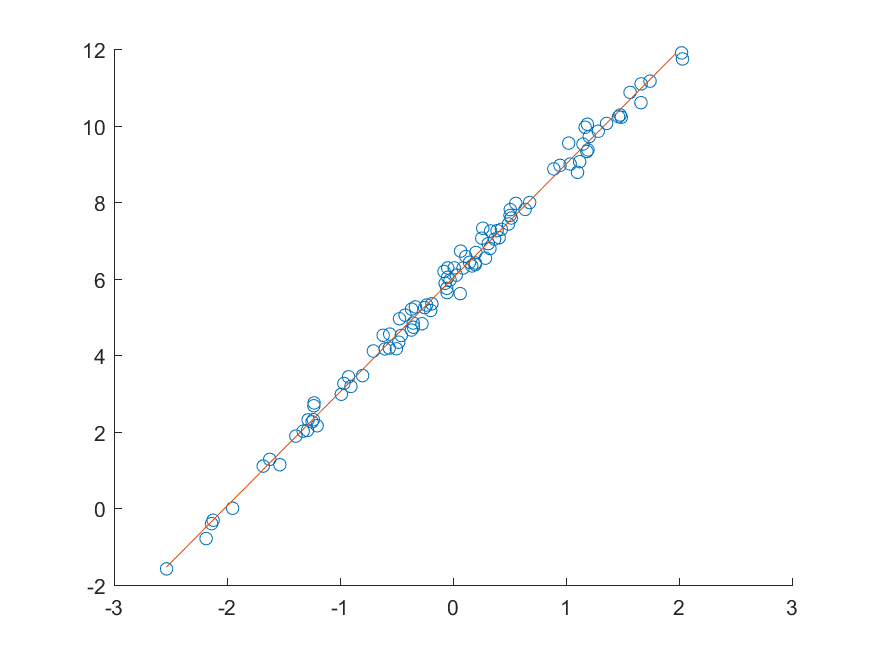
\includegraphics[width = 0.6\linewidth]{2-2-linear-100-0.5.png}
            \caption{Linear}
        \end{figure}

        \begin{figure}[H]
            \centering
            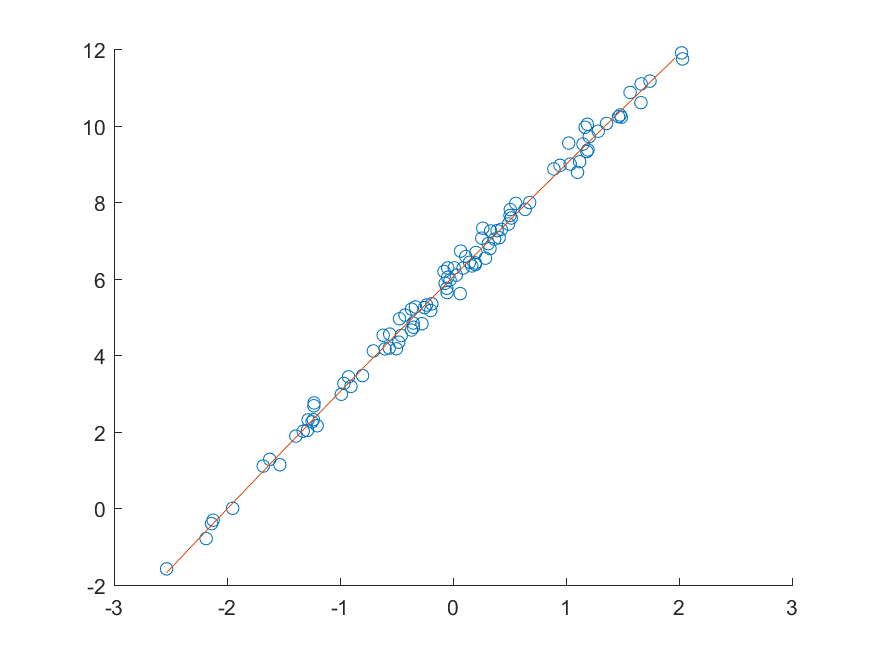
\includegraphics[width = 0.6\linewidth]{2-2-quadratic-100-0.5.png}
            \caption{Quadratic}
        \end{figure}

        \begin{figure}[H]
            \centering
            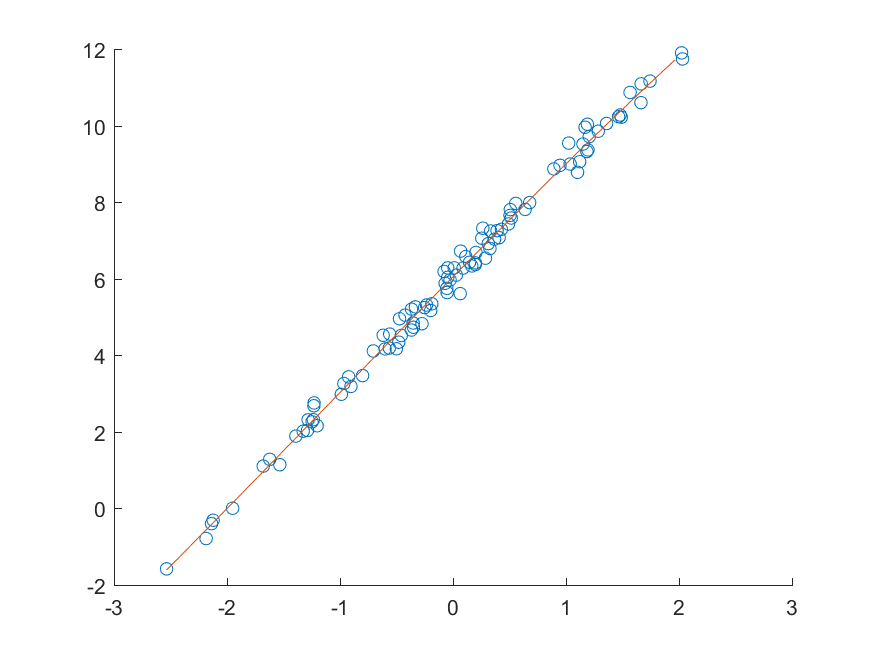
\includegraphics[width = 0.6\linewidth]{2-2-cubic-100-0.5.png}
            \caption{Cubic}
        \end{figure}

        Linear model (on testing set): $$\mathrm{RSS} = 6.6353, \quad \mathrm{RSS}/\mathrm{TSS} = 0.0014$$

        Quadratic model (on testing set): $$\mathrm{RSS} = 6.5180, \quad \mathrm{RSS}/\mathrm{TSS} = 0.0014$$

        Cubic model (on testing set): $$\mathrm{RSS} = 6.8288, \quad \mathrm{RSS}/\mathrm{TSS} = 0.0015$$
    }

    \subsection*{Case 3: $N=10$, $\sigma = 2$}
    {
        Linear model: $$\hat{y} = 5.6122 + 4.3460x ,\quad R^2 = 0.6779$$
        Quadratic model: $$\hat{y} = 5.7220 + 4.3487x - 0.0745x^2 ,\quad R^2 = 0.6783$$
        Cubic model: $$\hat{y} = 5.7827 + 2.3172x + 0.0726x^2 + 0.5700x^3 ,\quad R^2 = 0.6967$$

        \begin{figure}[H]
            \centering
            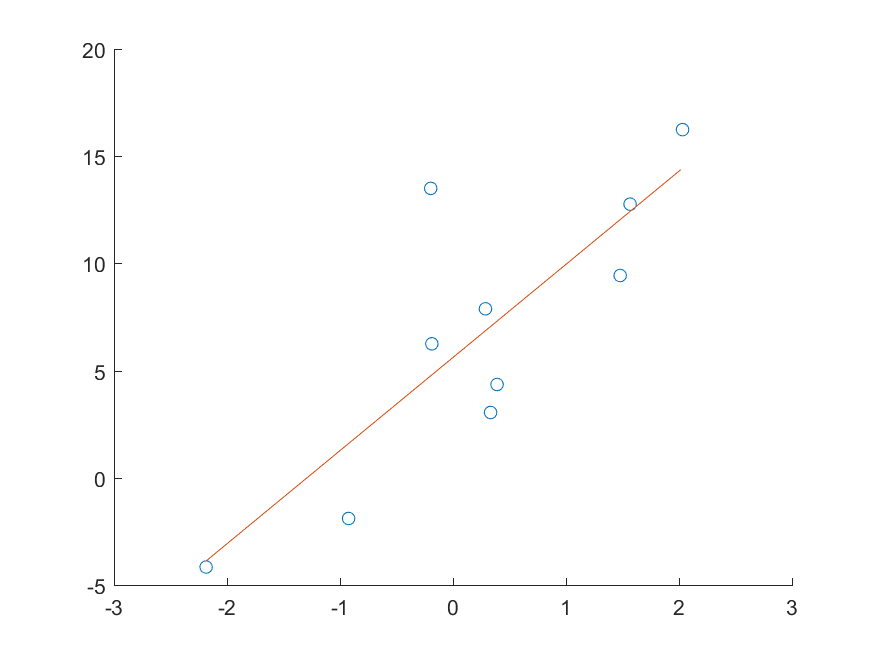
\includegraphics[width = 0.6\linewidth]{2-2-linear-10-2.0.png}
            \caption{Linear}
        \end{figure}

        \begin{figure}[H]
            \centering
            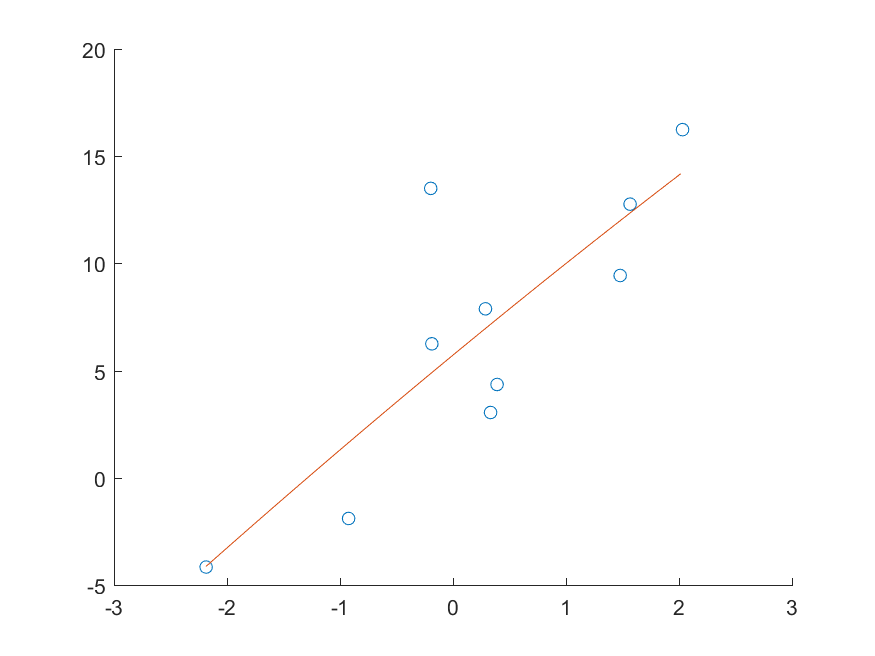
\includegraphics[width = 0.6\linewidth]{2-2-quadratic-10-2.0.png}
            \caption{Quadratic}
        \end{figure}

        \begin{figure}[H]
            \centering
            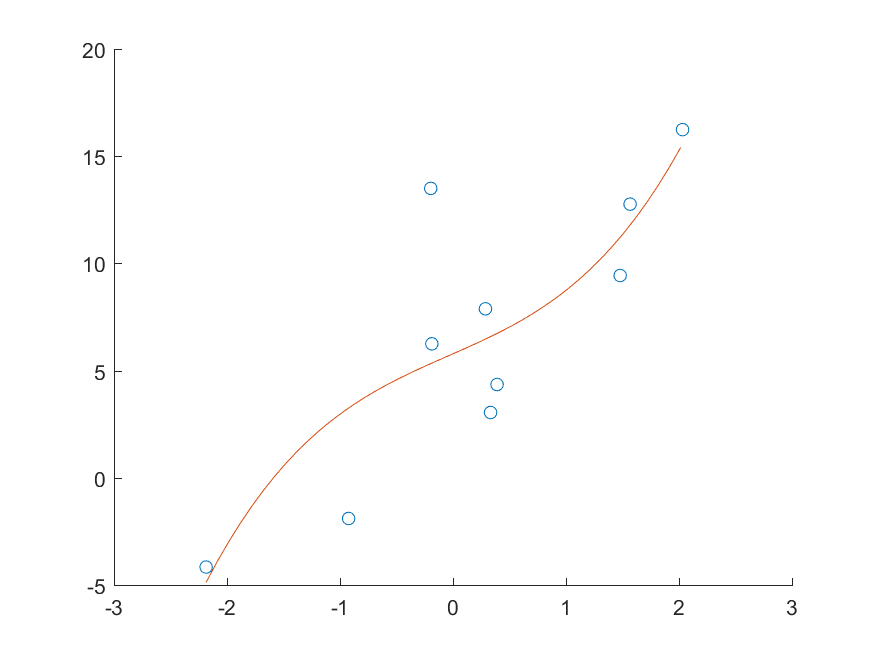
\includegraphics[width = 0.6\linewidth]{2-2-cubic-10-2.0.png}
            \caption{Cubic}     
        \end{figure}

        Linear model (on testing set): $$\mathrm{RSS} = 1914, \quad \mathrm{RSS}/\mathrm{TSS} = 0.3002$$

        Quadratic model (on testing set): $$\mathrm{RSS} = 1911, \quad \mathrm{RSS}/\mathrm{TSS} = 0.2996$$

        Cubic model (on testing set): $$\mathrm{RSS} = 1850, \quad \mathrm{RSS}/\mathrm{TSS} = 0.2901$$
    }

    \subsection*{Case 4: $N=100$, $\sigma = 2$}
    {
        Linear model: $$\hat{y} = 6.2433 + 2.6398x ,\quad R^2 = 0.3337$$
        Quadratic model: $$\hat{y} = 6.7499 + 2.5323x - 0.4973x^2 ,\quad R^2 = 0.3527$$
        Cubic model: $$\hat{y} = 6.8062 + 2.9781x - 0.5878x^2 - 0.1743x^3 ,\quad R^2 = 0.3560$$

        \begin{figure}[H]
            \centering
            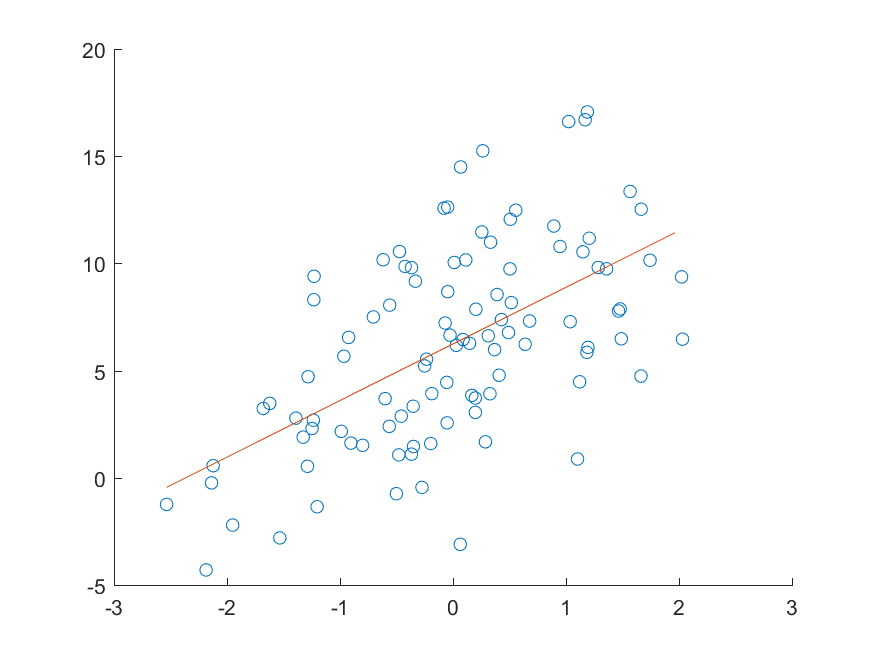
\includegraphics[width = 0.6\linewidth]{2-2-linear-100-2.0.png}
            \caption{Linear}
        \end{figure}

        \begin{figure}[H]
            \centering
            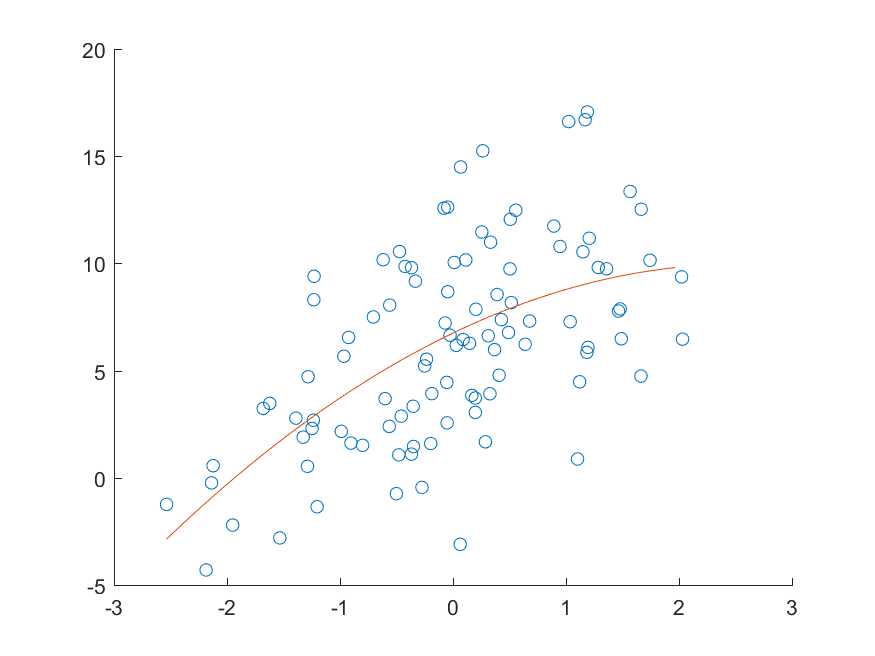
\includegraphics[width = 0.6\linewidth]{2-2-quadratic-100-2.0.png}
            \caption{Quadratic}
        \end{figure}

        \begin{figure}[H]
            \centering
            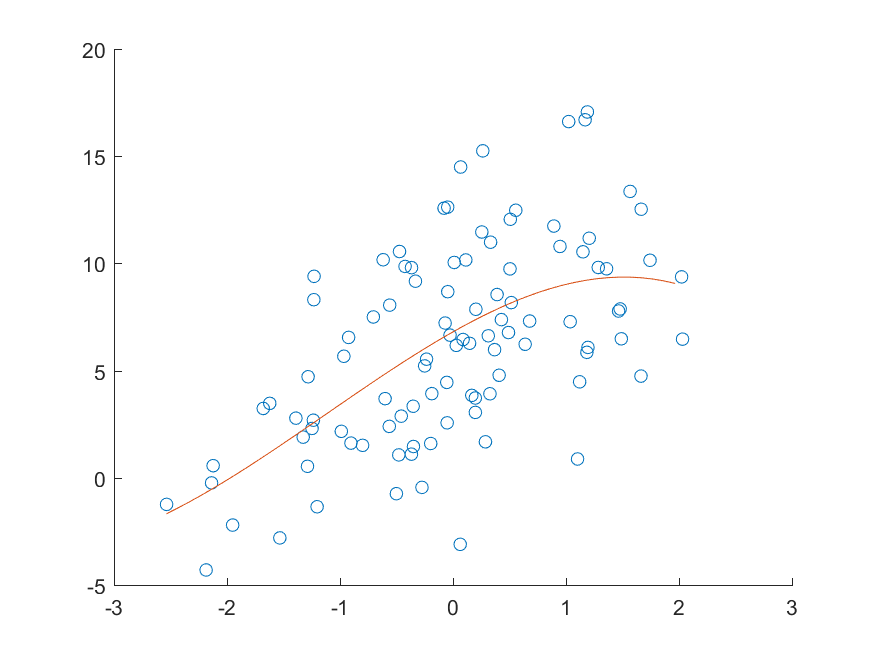
\includegraphics[width = 0.6\linewidth]{2-2-cubic-100-2.0.png}
            \caption{Cubic}
        \end{figure}

        Linear model (on testing set): $$\mathrm{RSS} = 1698, \quad \mathrm{RSS}/\mathrm{TSS} = 0.3049$$

        Quadratic model (on testing set): $$\mathrm{RSS} = 1668, \quad \mathrm{RSS}/\mathrm{TSS} = 0.2995$$

        Cubic model (on testing set): $$\mathrm{RSS} = 1748, \quad \mathrm{RSS}/\mathrm{TSS} = 0.3138$$
    }

    \subsection*{Conclusion}
    {
        \begin{itemize}
            \item (\emph{Complexity}) For $\sigma = 0.5$ (small), the data have good linearity, and therefore, the quadratic and the cubic terms are close to 0, which means the linear model is adequate to explain the data. For $\sigma = 2$ (large), however, the linear term has a small impact on the response, compared to the error term. In this circumstance, the quadratic and the cubic term is not neglegible. 

            \item For the 4 linear models, we have the following two tables:

            \begin{table}[!hbp]
                \begin{tabular}{|c|c|c|}
                \hline
                . & $N=10$ & $N=100$ \\
                \hline
                $\sigma=0.5$ & 0.9963 & 0.9939 \\
                \hline
                $\sigma=2$ & 0.6779 & 0.3337 \\
                \hline
                \end{tabular}
                \caption{$R^2$ on training set}
            \end{table}

            \begin{table}[!hbp]
                \begin{tabular}{|c|c|c|}
                \hline
                . & $N=10$ & $N=100$ \\
                \hline
                $\sigma=0.5$ & 0.9982 & 0.9986 \\
                \hline
                $\sigma=2$ & 0.6998 & 0.6951 \\
                \hline
                \end{tabular}
                \caption{$R^2$ on testing set}
            \end{table}

            We see the the $R^2$ on training set decreases dramatically with $N$ when $\sigma$ is large. 

            \item The training $R^2$ and the testing $R^2$ are different if they are based on different $N$s. Also, there is some stocasticity rooted in this experiment, which depends on the random seed.

        \end{itemize}
    }
}

\section*{Question 3}
{
    \subsection*{Without interactive terms}
    {
        $$\hat{y} = 726.0731 - 0.7537x_1 - 161.5401x_2 + 61.4084x_3, \quad R^2 = 0.2304$$.
        Plug in $x = (110, 3, 1)$, one has $$\hat{y} = 219.9584$$.
    }

    \subsection*{With interactive terms}
    {
        $$\hat{y} = 1929.531 - 4.7578x_1 - 924.4123x_2 + 3.6749x_3 + 2.5331x_1 x_2 - 137.5951x_2 x_3 - 0.2866x_3 x_1, \quad R^2 = 0.6050$$.
        Plug in $x = (110, 3, 1)$, one has $$\hat{y} = -607.9640$$.

        What is unique about the interactive terms is that they give a much higher $R^2$, which seems to better the explainability of the model. But the prediction value is negative, and makes an outlier. This condraction is caused by the collinearity of the raw data.
    }

    \subsection*{Alternative: Half interactive terms}
    {
        We propose an alternative method, in which we keep interactive terms except $x_1 x_2$. We find this trick works!

        $$\hat{y} = 669.9723 - 0.8563x_1 - 107.6020x_2 + 160.5363x_3 - 98.7687x_2 x_3 + 0.2065x_3 x_1, \quad R^2 = 0.2437$$.
        Plug in $x = (110, 3, 1)$, one has $$\hat{y} = 139.9174$$.

        In other words, we assume the the gene and the tumor size have no interactive effect. Under this assumption, we have a model with better $R^2$, and also give a reasonable prediction.
    }
}

\section*{Source Code}
{
    Please download the souece code from http://39.106.23.58/files/PR1\_2015011506.7z
}

\clearpage
\end{document}
    